\section{The Soul of a Woman}

\begin{quotex}
Adam knew Eve his wife \flright{\textsc{Genesis 4:1}}

\end{quotex}
Although he has copious notes, Cologero has been experiencing writer's block regarding his upcoming posts on the esoteric meaning of Romance. So he called me last night for help in overcoming that block. We had a long talk — or rather he talked and I listened — about Dante, Malory's novel on King Arthur, Donne's love poetry, Charles Williams, and a few other lesser known figures. Of course, this theme goes all the way back to his first writings about Lucinde\footnote{\url{http://www.gornahoor.net/?p=4}}.

Yet his concern was the lack of female authors who have written on the topic. As a psychologist, I could see that this concern was less intellectual and more personal. So I probed a little deeper. Sure enough, he revealed to me that he had never met a woman who understood what he is writing about. That has caused him to doubt the veracity, or at least the usefulness, of his research.

In exasperation, he informed me that several women have said that ``he gets them", yet they don't ``get him". I pointed out his naivety: man desires to know, woman desires to be known. It's in the Bible for heaven's sake. Over the years, he has engaged in voluminous correspondence, most of which he has shown me for analysis. I hope that this particular story will serve as an introduction to his topic and will free his blockage.

\begin{wrapfigure}{rt}{.37\textwidth}
 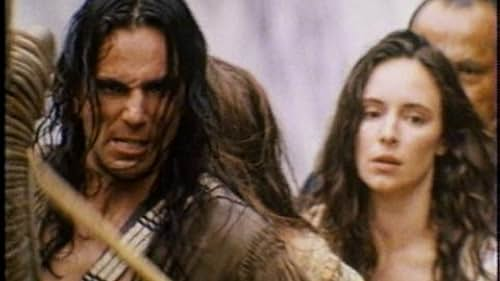
\includegraphics[scale=.25]{a20181204TheSoulofaWoman-img001.jpg} 
\end{wrapfigure}

Lila [not her real name] was young and pretty. She claimed to have a 160 IQ. Whether or not that is exactly true, I judged from her writings that she was certainly quite intelligent. Yet that is not the point, she still desired to be known. At one point, she sent him a tape of the movie \textit{Last of the Mohicans}\footnote{\url{https://www.imdb.com/title/tt0104691/?ref_=nv_sr_1}}, with a note that it was her favorite film. She asked for Cologero's opinion of it. Of course, Cologero thought it was a conversation starter, so this was his response:

\begin{quotex}
I actually finished the film yesterday. Clearly a magnificent movie, simultaneously a great adventure and a convincing love story, while demonstrating the variations of human character and the agony of the tough decisions we sometimes need to make.

I looked at Amazon and imdb … many people are captivated by this film. But what grabs Lila? What secret does she harbor, a secret she holds tight while longing for someone to pry it loose. It reminds me of one of those challenges the medieval knights had to conquer on the quest for the grail.

It must be more than the long hair and skill in the martial arts. The turning point for Cora came when they came upon the massacred family. Cora was distracted from her task and wanted to take time to give them a proper burial. Hawkeye, undeterred from his goal and brusquely dismissive of Cora's request, forces them to press on. She is angered by what she considers his cold-heartedness and moral failing. It is only when he brings her to see the situation in larger terms, that her infatuation begins. Suddenly, she is no longer the protected bourgeois daughter of a British officer. She is exposed to man's world with all its glory, cruelty, sinfulness, and stripped of its veneer of cultured, ``civilized" life. She also sees that a life with Duncan is part of that old, false world, and that real Love can only exist in the midst of the real world, with a man at home in that world, while still holding values that transcend it.

Hawkeye's and Cora's love is the beginning of their salvation. In the cave, the knowledge of Hawkeye's love fuels Cora's will to live through the faith he will keep his promise. For Hawkeye, all other concerns are secondary as he single-mindedly looks to rescue Cora. He also has the backing of his father and brother who demonstrate their loyalty. Yet love alone is insufficient and the couple needs to rely on the sacrifice of Duncan who, while not altogether the innocent victim, is yet made innocent by his love for Cora, a non-egoic love as he is willing to give her up for her own happiness.

Unlike Cain and Abel, Uncas dies for his brother … and for Cora. But he is unable to save Alice who, not understanding or loving like her sister, yields to her despair. As all the agents — the English, the settlers, the French, the Hurons, the Mohicans — act out their little parts on their stage, they are oblivious to the greater change they inadvertently are bringing about. Only the wise Chingachgook can see it all coming, sub specie aeternitatis, as it were. 

\end{quotex}
What Cologero didn't realize was that the question was not about the movie per se, but rather about Lila's soul. This was her response:

\begin{quotex}
Breathtaking. I am awestruck, and humbled. Thank you. I had wondered whether you really knew me. Now I know that you have seen into my very soul.

Yes, analytical, but not with a negative connotation, as in cold or calculating. What I was thinking about was this process you seem to have (correct me if I'm wrong), whereby you appear to step back, almost remove yourself from whatever it is, in order to observe, study, and contemplate an idea or situation (or a person, as it were). Then suddenly you turn around and have this uncanny ability to tell me what was in my head or in my heart before I'm even consciously aware of it. Case in point: The Last of the Mohicans. I didn't even know myself why it captivates me, so I was really curious as to what you'd come up with. You figured it out in no time flat, and you were exactly right. Nobody reads me like that, ever. And I guess I was thinking you'll apply those same abilities to look into my dreams, and they'll point up all my flaws. But it would seem they're all too readily apparent anyway. So I quit worrying about it. You're just too perceptive sometimes. It's a little scary! and I like it a lot — go figure. 

\end{quotex}
I think he is looking for a synthesis of identicals rather than of complementaries. Perhaps that is what Charles Williams meant when he wrote:

\begin{quotex}
Christ is the synthesis of the positive, and the Blessed Virgin of the receptive, side of man. 

\end{quotex}
At least, that is my understanding from Cologero's explanation.



\flrightit{Posted on 2018-12-04 by Teresa Chicalinda }

\begin{center}* * *\end{center}

\begin{footnotesize}\begin{sffamily}



\texttt{Alistair Fraser on 2018-12-05 at 04:32 said: }

Excellent, on the ``alice" character there was also something of a conscious choice being displayed prior to her demise , a perceived spiritual death at the hands of her new lovers killers or a physical death taking the same fall that her new lover was forced to take in her and others defence . She chooses the later.


\hfill

\texttt{Mikkel on 2018-12-08 at 19:28 said: }

Man wishes to know and woman to be known. One knows according to ability, ``Everything that is known is comprehended not according to its own nature, but according to the ability to know of those who do the knowing." not specifically studying the object of knowing, the other person. Woman pushes man to know himself through many ways in life, sometimes these are more `correct' than others, but the true need or goal here is a higher self-knowledge in order to know, it seems even that a woman instinctively dissuades or encourages a man through this, though not always correct, of course given a relationship the man has responsibility for his own discerning. The woman then can be known once the appropriate level of knowing is reached, and man then knows himself. By this, Man encapsulates knowing and being known in his own experience, masculine and feminine together. As well, by this woman may encapsulate knowing as man has brought her to herself and she is known by him.

It appears that there are corresponding levels of knowing of another person, physical, emotional, spiritual, the vehicle to the love understood in the Middle Ages discussed in the ``She who must be obeyed" article, ``This was Love at the spiritual and objective level, beyond both the carnal and the psychological level." Many relations today seem to want to be focused on a higher level than carnal or psychological, but people do not carry the type of responsibility appropriate (knowledge) to that higher level, causing much sadness and distress.

As well, man to know and woman to be known speaks even to the direct of which behavior can be seen, although typically these acts are studied mostly in children (Male children acting out externally, while female children withdrawing inwardly).


\end{sffamily}\end{footnotesize}
